\documentclass[a4paper,14pt]{extreport}

\usepackage[T2A]{fontenc}
\usepackage[utf8]{inputenc}
\usepackage[ukrainian]{babel}

\usepackage[unicode]{hyperref}
\hypersetup{colorlinks=false}

\usepackage{lastpage}
\usepackage{graphicx}
\usepackage{url}
\usepackage{listings}
\lstset{frame=single,basicstyle=\ttfamily\scriptsize,extendedchars=\true}

\usepackage{amssymb}

\newtheorem{lemma}{Лема}
\newtheorem{theorem}{Теорема}
\newtheorem{proposition}{Твердження}

\usepackage{multirow}
\usepackage{array}
\usepackage{longtable}

\usepackage{report/Styles/zvit}

% for literature
\usepackage{datetime}
\renewcommand{\dateseparator}{.}
% \newcommand{\todayiso}{\twodigit\day \dateseparator \twodigit\month \dateseparator \the\year}
\newcommand{\todayiso}{1.11.2018}

\begin{document}
% Need Linux package: scalable-cyrfonts-tex
\usefont{T2A}{ftm}{m}{n} %%% 

% Add C. to start of contents
\cftaddtitleline{toc}{part}{}{С.}

\frontmatter %%% <-- вимикаємо нумераці.

% Title page
\thispagestyle{empty}

\noindent УДК \quad 004.45; 004.2

\noindent \textnumero~держреєстрації 000U0001

% \noindent Інв. \textnumero


 \begin{centering}
  \linespread{1.1}
  \vspace{1em}

{Національна академія наук України

Інститут ....

1234 м. Київ-123, офіційна адреса, 40, тел. (044) 123-45-67}

  \vspace{1em}
  
\begin{tabular}{p{0.45\linewidth}p{0.01\linewidth}p{0.45\linewidth}}
\noindent ЗАТВЕРДЖУЮ & & \noindent ЗАТВЕРДЖУЮ \\
%left
Керівник Програми
академік НАН України 
& &
% Rignt
академік НАН України
\\

\rule{0.52\linewidth}{0pt}І.П.~Прізвище  & & \rule{0.52\linewidth}{0pt}І.П.~Прізвище\\

«\quad»\rule{0.35\linewidth}{0pt}20\quadр. & & «\quad»\rule{0.35\linewidth}{0pt}20\quadр.\\

\end{tabular}


  \vspace{0.5em}

ЗВІТ ЗА ПРОЕКТОМ

\textbf{«Розвиток шаблона звіту для пакету Latex}

\textbf{для формування звітів згідно з ДСТУ»}

виконаним в рамках цільової комплексної програми 

наукових досліджень НАН України

«Назва програми»

\begin{tabular}{p{0.45\linewidth}p{0.01\linewidth}p{0.45\linewidth}}
 & & \noindent ЗАТВЕРДЖУЮ \\

& &
% Rignt
Директор Інституту Назва \newline
НАН України
академік НАН України
\\

   & & \rule{0.52\linewidth}{0pt}І.П Прізвище\\

  & & «\quad»\rule{0.35\linewidth}{0pt}20\quadр.\\

\end{tabular}


\begin{tabular}{p{0.7\linewidth}p{0.25\linewidth}}

Керівник проекту & \\
Завідувач лабораторії & \\
кандидат технічних наук & І.П.~Прізвище \\

\end{tabular}

\vspace{3em}

  Київ -- 2018
  
% }
\end{centering}

{\small
\noindent Рукопис закінчено 02.11.2018 р.

\noindent Матеріали звіту розглянуто та затверджено Вченою радою Інституту
Назва,

\noindent протокол \textnumero 17 від 24.11.2018~р.

\vspace{1em}

\noindent Координаційна робоча група програми
}
% End of Titlepage


% \chapter*{ПЕРЕЛІК АВТОРІВ}
\chapter*{СПИСОК АВТОРІВ}


\begin{longtable}{p{0.45\linewidth}p{0.15\linewidth}p{0.3\linewidth}}
\textbf{Керівник НДР:} & &\\
Зав. відділом, & & \\
старший науковий співробітник, & & \\
доктор фізико-математичних наук & \rule{1\linewidth}{0.1pt} & ПІБ\\

\textbf{Відповідальні виконавці:} & &\\
Старший науковий співробітник & & \\
кандидат технічних наук & \rule{1\linewidth}{0.1pt} & ПІБ\\
Старший науковий співробітник & & \\
кандидат фізико-математичних наук & \rule{1\linewidth}{0.1pt} & ПІБ\\

\textbf{Виконавці:} & & \\
Молодший науковий співробітник & \rule{1\linewidth}{0.1pt} & ПІБ\\
Молодший науковий співробітник & \rule{1\linewidth}{0.1pt} & ПІБ\\
\end{longtable}

\chapter*{РЕФЕРАТ}

Звіт по НДР: \pageref{LastPage}~с., \total{citenum}~джерел, 
\total{tablenum}~табл, \total{figurenum}~рис.

% \vspace{1cm}
Latex, Шаблон, Звіт, ДСТУ


Метою проекту є розробка шаблону для звітів. 

Завдання проекту – якісь завдання

Головними результатами проекту є шаблон і його застосування. Основні результати виконання проекту:

\begin{itemize}
\item модернізовано;
\item створено;
\item розроблено;
\item забезпечено;
\item проведено.
\end{itemize}






\tableofcontents

\chapter{ПЕРЕЛІК СКОРОЧЕНЬ, УМОВНИХ ПОЗНАК}
% За алфавітом

\begin{description}
\item[AMD64/EM64T] --- 64-розрядна мікропроцесорна архітектура
\item[Cloud computing] --- технологія обробки даних на базі Internet-сервісів
\item[CPU] --- центральний процесор
\item[Gbps] --- гігабіт за секунду
\item[GHz] --- гігагерц
\item[GPU] --- графічний процесор
\item[IBM] --- американська корпорація, виробник обчислювальної техніки
\item[Infiniband, Myrinet, Quadrix] --- високопродуктивні мережі передачі даних
\item[Linpack] --- бібліотека програм для тестування комп'ютерів
\item[Linux] --- UNIX- подібна операційна система
\item[Lustre] --- розподілена файлова система
\item[RAID] --- надлишковий масив незалежних дисків
\item[RAM] --- запам'ятовуючий пристрій з довільним доступом
\item[SLURM] --- менеджер ресурсів кластера
\item[Web-портал] --- Web-сайт, що надає користувачам різноманітні інтерактивні сервіси
\item[БПЗ] --- базове програмне забезпечення
\item[ЕОМ] --- електронна обчислювальна машина
\item[ІК НАНУ] --- Інститут кібернетики ім. В.М.~Глушкова НАН України
\item[ОС] --- операційна система
\item[ПЗ] --- програмне забезпечення
\item[СКІТ] --- суперкомп'ютер інформаційних технологій
\item[СЛАР] --- система лінійних алгебраїчних рівнянь
\item[МСЕ] --- метод скінченних елементів
\item[суперкомп'ютер] --- обчислювальна система, яка має визначні характеристики продуктивності у порівнянні з комп'ютерами загального вжитку, у роботі терміни ``суперкомп'ютер'', ``обчислювальний кластер'', ``обчислювальний комплекс'' використовуються як синоніми
\item[гібридний вузол] --- обчислювальний вузол, в якому для обрахунків використовуються як універсальні процесори, так і спеціалізовані акселератори
\end{description}
\chapter{ВСТУП}

Ресурсний центр УНГ на основі суперкомп’ютерного комплексу СКІТ є найбільшим обчислюівальним центром в Україні, що надає науковцям НАН України можливості для виконання складних ресурсоємних науково-технічних розрахунків, і є однією з ключових складових УНГ, що забезпечує сервіси з обчислення та збереження даних для гріду в цілому.   Використання ресурсів СКІТ через хмарну підсистему, грід та безпосередньо у кластері допомагає науковими інститутам отримувати нові наукові результати та створювати цілу нові технології в широкому спектрі дисциплін: від генетики до лінгвістики. Проект присвячено розвитку ресурсного центру як інтегрованої складової частини національної грід-інфраструктури.

Архітектурні рішення, створені і впроваджені в процесі розробки ресурсного центру СКІТ, використовуються при побудові інших вітчизняних та закордонних обчислювальних систем.

І так далі про актуальність і важливість.

Результати проекту впроваджено у Ресурсному центрі Українського національного гріду. Розроблене системне та прикладне програмне забезпечення доступне для широкого загалу користувачів з НАН і МОН України. 


\mainmatter %% вмикаємо нумераці.

\chapter{РОЗВИТОК КЛАСТЕРА СКІТ}
% 1 Постановка та актуальність тематичної задачі або задач.
% 2 Отримані наукові результати (з посиланнями на перелік статей, що опубліковані за тематикою проекту). Додати в тексті схеми, рисунки, скріншоти.

% \section{Розвиток ресурсного центру УНГ на основі суперкомп'ютера СКІТ}

Важливим фактором розвитку і популяризації грід-технологій в Україні є наявність значних обчислювальних ресурсів у грід-інфраструктурі УНГ. Зокрема цього вимагає задача інтеграції України в європейський грід-простір~\cite{erevan-grid-2013}. На сьогоднішній день комплекс СКІТ надає в УНГ найбільший обсяг як обчислювальних ресурсів, так і ресурсів збереження. Проте розвиток технологій вимагає постійного оновлення як обладнання, так і системного та прикладного програмного забезпечення.


\section{Забезпечення надійності основних сервісів суперкомп'ютера}

В 2015 році EGI підвищило вимоги до надійності сервісів грід-сайтів. Тепер показник їх доступності (відношення часу, коли сервіси сайта проходять тести без помилок, до всього часу) має бути не меншим за 95\%. Тому постала задача підвищення надійності апаратної складової грід-сервісів, а також їх мобільності, тобто можливості швидкого перенесення всіх складових грід-сервісів кластера з несправного обладнання на справне.

Першим етапом цих робіт було перенесення всіх грід-серверів у віртуальні контейнери.  Було створено дослідний сервер-носій, на якому розміщувались всі віртуальні машини, необхідні для роботи ARC.

Дослідна експлуатація протягом 2014--2018 рр показала беззаперечні переваги такого рішення:

\begin{itemize}
\item можливість живої міграції, тобто перенесення віртуальної машини на резервний сервер-носій без перерви у наданні сервісів.
\item можливість "м'якого" оновлення проміжного ПЗ гріда. Оновлення відбувається не у робочій віртуальній машині, а у її копії. Коли оновлення готове, одна машина вимикається, а інша вмикається. А при появі якихось проблем з новим ПЗ, попередні версії сервісів відновлюються за декілька секунд.
\item відсутність жорсткої прив'язки до обладнання дозволила полегшити проведення планового та непланового технічного обслуговування серверів, і відповідно, підвищити надійність.                                                                                                                                                                              \end{itemize}

У 2016 році було проведено роботи з віртуалізації обчислювальних вузлів з черг моніторингу і діагностики.

Крім того, були оновлені ключові елементи інфраструктури -- кондиціонери та системи безперебійног живлення, що дозволить і надалі підтримувати високі стандарти надійності грід-сервісів.


\section{Віртуалізація вузлів діагностичного розділу грід-сайта}

До діагностичного розділу кластера грід-сайта входять вузли та черги, що виконують задачі систем моніторингу гріда. Ці задачі є придатними до віртуалізації, оскільки не потребують значних об'ємів пам'яті та процесорних ресурсів.  Це зумовлюють два фактори: 
\begin{enumerate}
\item підвищені вимоги до надійності цих вузлів, оскільки результати тестів на цих вузлах визначають оцінки кластера вцілому;
\item мінімальне обчислювальне навантаження при прохдженні теста.
\end{enumerate}

Було проведено аналіз технологій віртуалізації та виконано перенесення обчислювальних вузлів черги моніторингу у віртуальні контейнери. І таким чином зроблено внесок у вирішення задач підвищення енергоефективності обчислювального комплекса та підвищення його надійності.


\section{Інтеграція грід-сайта СКІТ до проекту ALICE}

Проект ALICE є одним з основних проектів Великого адронного коллайдера. Задачі обробки даних екперимента розподіляються по обчислювальним кластерам за допомогою грід-технологій та спеціалізованих віртуальних машин VOBOX. 

У роботі виконано роботи з узгодження системного ПЗ кластера СКІТ з потребами проекта ALICE, виконано встановлення та налагодження віртуального контейнера з сервісами VOBOX, отримання необхідних сертифікатів.

\begin{figure}
 \centering
 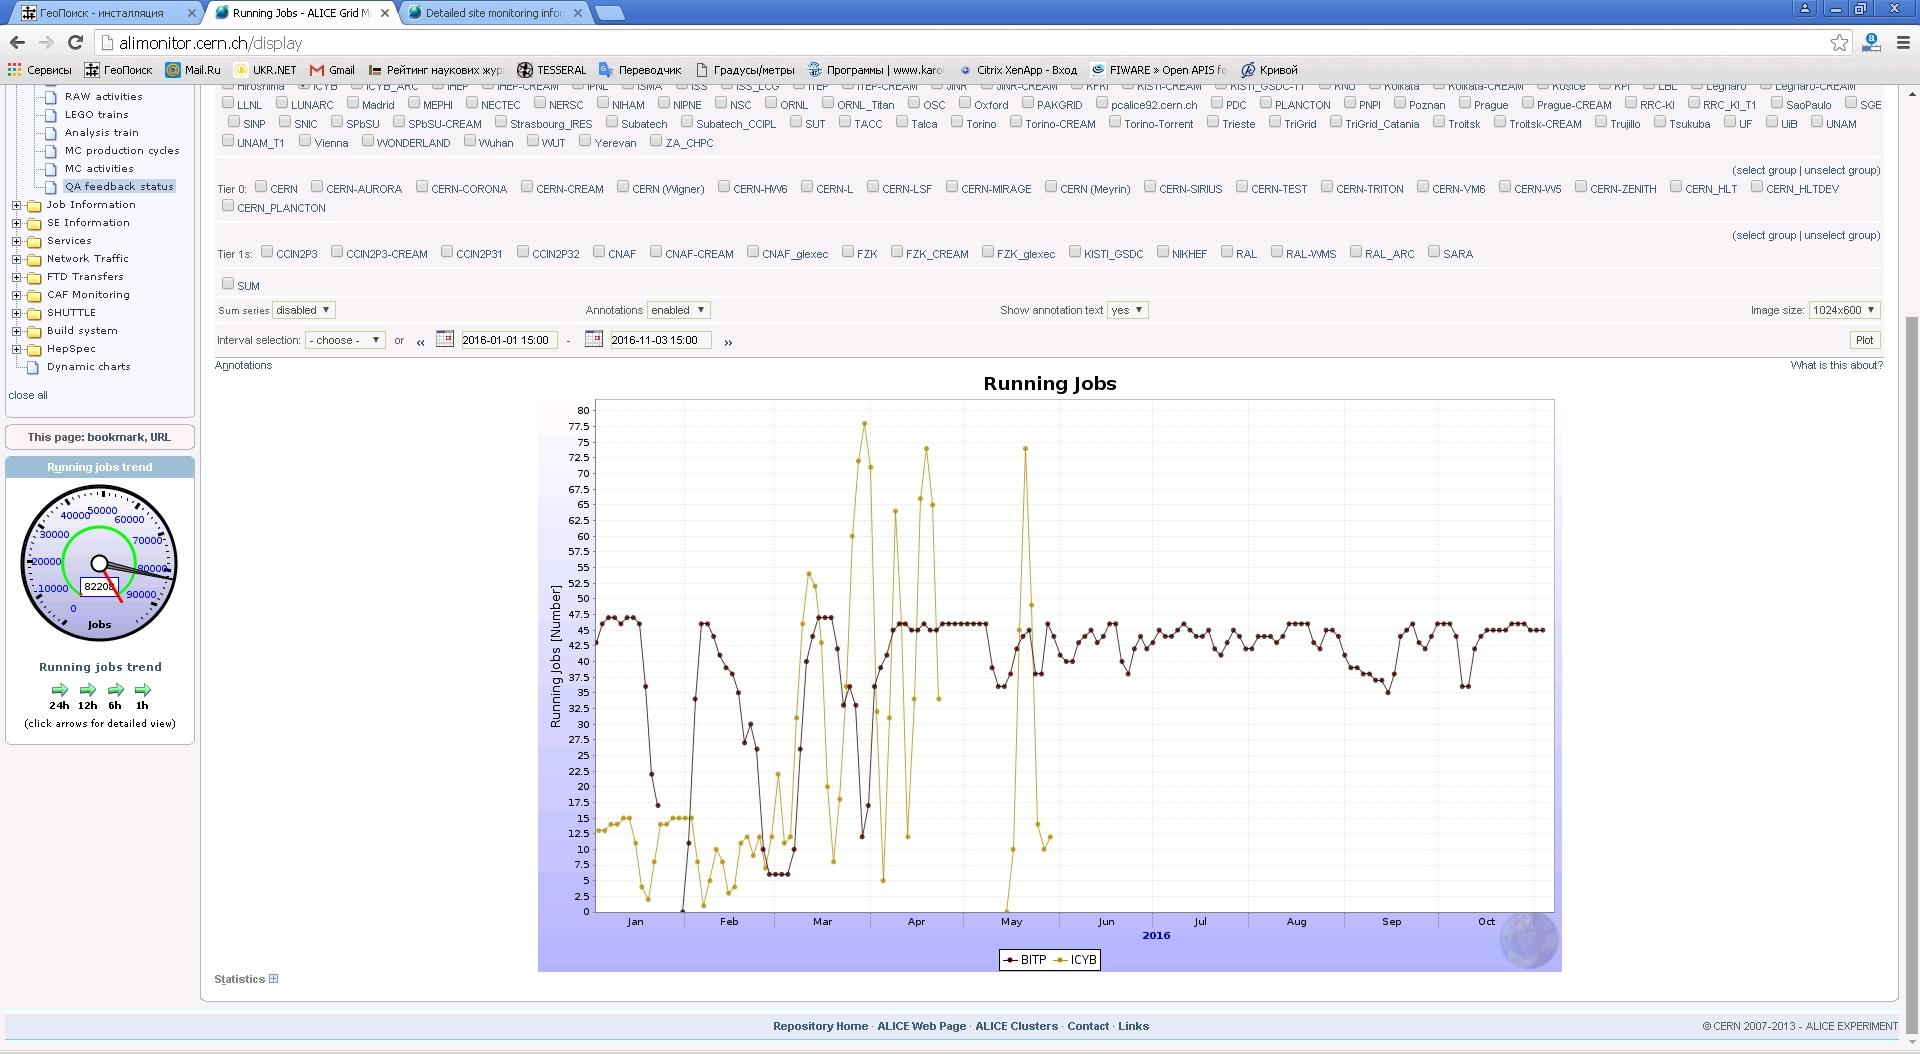
\includegraphics[width=14cm]{report/Illustrations/alice-stats.jpg} 
 \caption{Моніторинг проекта ALICE}
 \label{fig:alicemon}
\end{figure}

Крім того, проведено тестування роботи кластера з потоком реальних задач ALICE~\ref{fig:alicemon}.




\chapter{РОЗВИТОК АРХІТЕКТУРИ}

\section{Аналіз роботи суперкомп'ютерів сімейства СКІТ}

Обчислювальні кластери сімейства СКІТ є несерійними дослідними системами, які були побудовані на найкращій технологічній основі свого часу, та втілили оригінальні вітчизняні розробки в області системного програмного забезпечення та бібліотек обчислювальної математики.

У даній роботі ми провели ретроспективний аналіз розвитку архітектури СКІТ та впорядкували статистичні дані користування кластерами.

Аналіз статистики роботи користувачів проводиться у багатьох великих суперкомп’ютерних центрах~\cite{haozhang,scit10anniv}. Так, у роботі~\cite{haozhang} проведено подібний  аналіз для Суперкомп’ютера Кракен Оакріджської лабораторії, США. Попри різницю у кількості ядер і географічне розташування. Ці дві системи мають схожу структуру обчислювальних задач за областями науки, та параметри розподілу обчислювальних задач.

\subsection{Еволюція архітектури проекту СКІТ}

Архітектура кластерів сімейства СКІТ пройшла п'ять основних етапів, показаних в табл.~\ref{tab:scit}.

\begin{table}[htb]
  \begin{center}
    \caption{Продуктивність кластерів сімейства СКІТ}
    \begin{tabular}{|l|c|c|c|}
      \hline
Рік & Назва & Кількість ядер & Linpack, ТФлопс \\
\hline
2003 & СКІТ-0 & 4   & 0.02 \\
2004 & СКІТ-1 & 48  & 0.19 \\
2005 & СКІТ-2 & 64  & 0.28 \\
2007 & СКІТ-3 & 725 & 5.3 \\
2012 & СКІТ-4 & 448 & 18 \\
\hline
    \end{tabular}
    \label{tab:scit}
  \end{center}
\end{table}


Перший дослідний зразок обчислювального кластера СКІТ-0 було створено у 2003 - 2004 роках. Основні ідеї проекту описано у роботах авторів~\cite{scit-project-art}. Кластер мав 4 вузли на AMD Duron 800, інтерконект 100Мб Fast Ethernet, сховище даних мало об'єм 160 ГБ на основі масиву RAID-1.

Оригінальною особливістю цього кластера, яка відрізняла його від класичної архітектури Beowulf, був бездисковий принцип завантаження, коли всі вузли є клонами, завантаженими з одного образу операційної системи. Це дозволило полегшити адміністрування та швидко і синхронно вносити зміни у системне та прикладне програмне забезпечення. На цьому кластері було відпрацьовано таке архітектурне рішення як спільне дискове сховище для домашніх тек користувачів, що одночасно монтувалось на всі вузли кластера. Ці рішення залишились у наступних проектах майже без змін. СКІТ-0 не мав спеціалізованої системи керування, системи черг. MPI задачі запускались з візуальним контролем зайнятості вузлів. На цьому кластері було вирішено низку важливих задач моделювання зміни клімату, фільтрації ґрунтів та розрахунку міцності конструкцій.
У 2004-2006 рр. майже одночасно було створено два принципово різних кластера: СКІТ-1 та СКІТ-2, основні ідеї створення описані авторами у статтях~\cite{cluster-art,scit-art,polzovatel-int-art}.  

СКІТ-1 (13 позиція у 1-й редакції рейтингу Top50 суперкомп’ютерів СНД~\cite{top50} від 07.12.2004) мав 24 вузли на процесорах Intel Xeon з 32-бітною архітектурою i386, інтерконект Infiniband SDR. СКІТ-2 мав 32 вузли з інноваційними процесорами Intel Itanium-2 з 64-бітною архітектурою ia64. Встановлений інтерконект Dophinics SCI мав нижчу латентність і вищу швидкодію у порівнянні з Infiniband, але мав проблеми з надійністю.  Кластери мали власні керівні сервери і спільну систему збереження даних об'ємом 480ГБ на основі контролерів MegaRAID типу RAID6.

Для керування ресурсами кластерів була розроблена оригінальна система керування MVS, яка формувала чергу обчислювальних задач, надавала зручний діалоговий інтерфейс користувача та засоби задання пріоритетів задач, в системі був денний і нічний режим роботи. У денному режимі кластер ставив на обрахунок тільки короткі задачі, а великі багатодобові задачі починали обрахунок вночі. Таким чином звільнялись ресурси для швидкої обробки коротких задач у робочий час.

Кластер СКІТ-2 (8 позиція у 2-й редакції рейтингу Top50 суперкомп’ютерів СНД від 05.04.2005) мав передову технологію IPMI-1.1, яка дозволяла керувати живленням вузлів та контролювати стан обладнання. Ця система згодом з'явилась і стала основною на платформах Intel х64. 

В 2007-2008 рр було створено кластер СКІТ-3 (5 позиція у 6-й редакції рейтингу Top50 суперкомп’ютерів СНД від 11.04.2007), концепція якого описана авторами у статті~\cite{50anniv-art}. Кластер мав 125 вузлів та 725 процесорних ядер. В основу кластера лягли новітні на той момент 64-бітні процесори 2-ядерний Intel Xeon 5160 3.0 ГГц та  4-ядерний Xeon E5345 2.33 ГГц з архітектурою x64. Мережею передачі даних став Infiniband DDR, зі швидкодією 20~Гб/с.    

Важливим кроком був перехід на паралельну файлову систему Lustre при побудові системи збереження даних. Ця файлова система має у складі набір вузлів збереження, які підтримують одночасну паралельну роботу з вузлами кластера, що дозволило досягнути швидкодії дискової системи понад 1ГБ/с у паралельних обчислювальних задачах, а об'єм збільшити до 33 ТБ (табл.~\ref{tab:storage}).


\begin{table}[htb]
  \begin{center}
    \caption{Об'єм сховища на основі паралельної файлової системи Lustre}
    \begin{tabular}{|l|c|c|c|}
      \hline
Рік & Об’єм, ТБ \\
      \hline
2006 & 0.16 \\
2007 & 0.6 \\
2008 & 5.3 \\
2009 & 17 \\
2010 & 33 \\
2012 & 80 \\
2015 & 120 \\
2016 & 170 \\
2017 & 120 \\
\hline
    \end{tabular}
    \label{tab:storage}
  \end{center}
\end{table}


В якості системи керування обчислювальними ресурсами було обрано менеджер ресурсів SLURM, який надавав гнучкість у контролі за потоком задач та обчислювальними вузлами та простоту конфігурації.

У 2013 році було створено кластер СКІТ-4 [7,8]. Кластер має 28 вузлів та 448 процесорних ядер. Визначною зміною в архітектурі стало використання гібридних обчислювальних вузлів, в яких крім  процесорів Intel Xeon E5-2600 2.6 ГГц з архітектурою x64 використовувались графічні прискорювачі NVidia Tesla M2075. 

Графічні прискорювачі дозволяють частину обчислювального алгоритму виконувати на власних спеціалізованих процесорах, яких є значна кількість на одній платі (448 для M2075, 1344 на одному вузлі). У реальній роботі прискорювачі показали себе неоднозначно. З одного боку в спеціально перероблених для цього алгоритмах досягалась висока продуктивність. З іншого боку, більшість програмних пакетів, які використовуються користувачами СКІТ не мають GPU версій, а ті, що підтримують, мають реалізацію лише деякої підмножини алгоритмів пакету. 

Кластер СКІТ-5 має стати наступною системою в сімействі, архітектура його наразі розробляється і досліджуються різні перспективні рішення. Це перехід на SSD накопичувачі у системі збереження даних, дослідження постійних запам'ятовувальних пристроїв на технології NVMe, дослідження прискорювачів Intel XeonPhi, перехід від RAID масивів до файлових систем нового покоління, таких як ZFS тощо.

\subsection{Статистика надійності обладнання СКІТ}

Апаратна архітектура суперкомп’ютерів зазвичай добре висвітлена у анонсах чергових модернізацій. Однак майже не публікується даних щодо надійності обладнання протягом тривалого часу. Насамперед це пов’язано з високим темпом модернізації американських та європейських обчислювальних систем.

За десять років на основі журналу ремонтів СКІТ накопичилась певна статистика щодо обладнання. Звичайно, дане обладнання вже давно застаріло і воно не може бути орієнтиром при створенні нового кластера, але дає деяке уявлення, як веде себе кластер протягом часу. 

Вузли кластерів СКІТ побудовані на кількох типах платформ:

\begin{itemize}
\item Tyan S5370;
\item Supermicro TWIN X8DTT-F;
\item Supermicro GPU Nvidia Tesla M2050;
\item HP Proiant SL250 Gen 8 з GPU Nvidia Tesla M2075;
\item HP Proliant SL230 Gen 8.
\end{itemize}

За нашою статистикою, надійність платформ є у прямій відповідності до класу виробника. Найгірше себе показали платформи Tyan, на яких одразу виникли проблеми і за 9 років вийшло з ладу 10\%. До Supermicro суттєвих зауважень немає, втрати за 8 років склали 5\%. Найкраще себе показав виробник класу A., Hewlett Pakkard,  у якого за 4 роки обійшлося без втрат. 

За обладнанням вузлів, основні проблеми є з материнськими платами, платами IPMI, та пам'яттю. Найбільш надійними виявились процесори Intel Xeon різних серій, обійшлося без втрат.

Використання десктопних материнських плат в серверах та обчислювальних вузлах. У 2012-2013 роки ми проводили дослідження можливості використання десктопних компонентів у вузлах та серверах, оскільки вони є набагато дешевшими за серверні. Було створено кілька вузлів з материнськими платами на Intel Core i5, з прискорювачами Radeon 9660, блоками живлення на 700 Вт. Їх робота показала, що така концепція не виправдана, оскільки більшість обладнання не витримала роботу в режимі 24/7 * 365 і вийшла з ладу протягом року.

Жорсткі диски у сховищі даних на базі ОС Lustre. Диски у більшості своїй мають обмежений термін служби. Ми використовували наступні серії:
\begin{itemize}
\item Hitachi Deskstar 500 ГБ;
\item WD 2 ТБ;
\item Seagate 3ТБ;
\item Hitachi Deskstar NAS 6ТБ.
\end{itemize}

Hitachi 500 показали себе з найкращої сторони, за 8 років експлуатації вийшло з ладу лише близько 5\% дисків, інші морально застаріли і були виведені з основної конфігурації, але продовжують працювати на менш відповідальних ділянках.

WD були енергоощадливої десктопної лінійки, Seagate теж недорогої десктопної серії, і їх термін служби склав 3 роки, скільки прописано в гарантії, після чого 80\% їх вийшло з ладу.

Щодо Hitachi Hitach Deskstar 6 ТБ поки є лише пів року статистики, ніяких проблем не виявлено.

Виходячи з наведеного, необхідним є постійне підтримання резерву у 2-5 дисків кожного типу, що використовуються у системі збереження.

Надійність комутаторів мережі Ethernet та контролерів мережі Infiniband в цілому відповідає тому, що це технології на передньому краї науки. З 17 комутаторів на 10 років вийшло з ладу 2 і приблизно 3\% мережевих контролерів у вузлах.

У якості Ethernet обладнання використовувались  керовані комутатори HP ProCurve та DLink різних серій. Комутатори високого класу HP ProCurve показали себе з найкращої сторони, а все інше виходило з ладу чи починало мати дефекти роботи після 3-5 років експлуатації. 

Джерела безперебійного живлення. Використовувались APC Smart UPS різних серій. Ці блоки безперебійного живлення виявились в цілому надійними, з 20 блоків за 10 років вийшов з ладу лише один, якщо не враховувати вихід з ладу батарей. Батареї є слабким місцем і працюють в середньому лише 5 років, після чого потребують заміни.

\subsection{Статистика роботи комплексу СКІТ}

Для забезпечення ефективного функціонування кластерного комплексу СКІТ та його пристосування до потреб користувачів, надзвичайно важливо проводити збір та аналіз статистики роботи кластера. Завдяки цій важливій інформації можливо  визначити структуру обчислювальних задач, встановити, якому прикладному програмному забезпеченню необхідно найбільше приділяти увагу, коригувати різноманітні параметри черги задач, створювати нові глобальні профілі запуску задач у порталі кластерних обчислень. Також дуже актуальним є контроль за використанням кластерних ресурсів окремими користувачами або організаціями.

При обробці даних від менеджера ресурсів кластеру можливо отримати наступні статистичні показники використання кластера за даний певний період:
\begin{itemize}
 \item Кількість задач, які були запущені на виконання. Цей показник показує активність використання кластера користувачами в кількісному вираженні.
 \item Структура задач за статусом завершення як в абсолютних, так і відносних величинах. Дозволяє визначити, яка частка задач серед поставлених у чергу виконана успішно.
 \item Середня тривалість однієї задачі. Визначає характер використання кластера: екстенсивно чи інтенсивно.
 \item Сумарне завантаження кластеру в процесоро-хвилинах, визначається як сума часу виконання кожної задачі, помноженої на кількість зайнятих нею процесорів. 
\end{itemize}


Окремо необхідно розраховувати статистичні дані як по кластеру в цілому, так і в розрізі користувачів та організації, при цьому додатково обраховуються наступні параметри:
\begin{itemize}
 \item Частка задач окремого користувача чи організації у загальній кількості задач за період, дозволяє визначити його активність по запуску задач у порівнянні з іншими користувачами. 
 \item Частка завантаження кластера користувачем у сумарному завантаженні кластеру, дозволяє відстежити основних споживачів кластерних ресурсів СКІТ.
\end{itemize}

Загалом, за період 2005-2016 рр кластери СКІТ надали 11,8 млн процесоро-годин обчислювальних ресурсів, виконавши більше 70 тис. задач користувачів. Зведена статистика за роками наведена у табл.~\ref{tab:usage}.


\begin{table}[htb]
  \begin{center}
    \caption{Робота кластерів СКІТ за 2006-2015 роки}
    \begin{tabular}{|l|c|c|c|}
      \hline
Рік & Кількість задач & Процесоро-години, тис & Середній час виконання, хв \\
      \hline
2006 & 1050 & 2,3 & 34 \\
2007 & 12017 & 207,8 & 27 \\
2008 & 11043 & 107,2 & 142 \\
2009 & 11475 & 2440,7 & 479 \\
2010 & 17251 & 2870,1 & 310 \\
2011 & 16334 & 2340,2 & 300 \\
2012 & 12784 & 1845,3 & 320 \\
2013 & 9678 & 877,8 & 373 \\
2014 & 7107 & 1039,2 & 1049 \\
2015 & 1548 & 47,7 & 425 \\
\hline
Всього & 71169 & 11778,2 & \\
\hline
    \end{tabular}
    \label{tab:usage}
  \end{center}
\end{table}


Найбільше обчислювальних ресурсів кластери надавали у докризові 2009-2010, надалі кількість процесоро-годин зменшувалась, що спричинене економічними факторами, насамперед обмеженим фінансуванням витрат на електроенергію.


Середня річна кількість активних користувачів складає 50 чоловік. Зведену статистику за типами обчислювальних задач охарактеризуємо наступним чином:

\begin{enumerate}
 \item Квантово-хімічні розрахунки, близько 100 тис процесоро-годин на рік: дослідження активних центрів біологічних молекул, пошук нових ліків.
 \item  Молекулярна динаміка, близько 100 тис процесоро-годин на рік: дослідження органічних молекул із складною тривимірною структурою: білків, ДНК, тощо.
 \item  Алгебра і теорія чисел, близько 10 тис процесоро-годин на рік: чисельні експерименти для доведення теорем, підтвердження гіпотез.
 \item  Обробка результатів експерименту ALICE на LHC, 10 тис процесоро-годин  на рік.
 \item  Розрахункові задачі гідродинаміки, 25 тис процесоро-годин на рік.
\end{enumerate}


За період в десять років в такій динамічній області як обчислювальні системи змінилось багато трендів: з’явились і занепали грід-технології, з’явились і потужно заявили про себе хмарні системи. Однак суперкомп’ютери залишаються  основним  інструментом вирішення складних науково-технічних задач. 
Суперкомп’ютерний комплекс СКІТ є найбільшим обчислювальним центром України, орієнтованим на вирішення широкого кола наукових задач. Доступ до нього здійснюється як через веб-інтерфейс на офіційному сайті~\cite{ic}, так і традиційним SSH. Спеціалісти Інституту кібернетики проводять дослідження в області архітектури високопродуктивних обчислювальних систем, проводять розробку засобів їх керування та діагностики. 


\backmatter

\chapter{ВИСНОВКИ}

За результатами виконання проекту можна зробити наступні висновки.

\begin{enumerate}
\item Результат.
\item Результат.
\end{enumerate}



\clearpage
\addcontentsline{toc}{chapter}{ПЕРЕЛІК ДЖЕРЕЛ ПОСИЛАННЯ}
\bibliographystyle{gost780}
\bibliography{literatura}

% enable numbering in appendices
% \mainmatter
\appendix

%Fix Cyrillic letters in appendix numbering
\makeatletter
% Fix Title format
\gdef\thechapter{\@Asbuk\c@chapter}
\makeatother
\titleformat{\chapter}
  {\normalfont \centering}
  {ДОДАТОК~\Asbuk{chapter}~}{0pt}{}
\titlespacing{\chapter}{0cm}{0em}{3em}


\end{document}
